\newpage
\section{Results}
\subsection{The Change in Aerosol Concentrations}
After applying the high-pressure blocking detection method to the data from Vavihill and Malmö for the entire period, a total of 247 high-pressure blocking events were identified between November 27, 1995 and September 22, 2024. For Vavihill 128 high-pressure blocking events of the original 247 were removed due to insufficient \PM data, as a filter requiring 85\% data coverage was applied. This left 119 relevant high-pressure blocking events. For Malmö 58 high-pressure blocking events were removed due to insufficient \PM data, again applying the 85\% data coverage filter. This resulted in 189 relevant high-pressure blocking events. An example plot showing periods of high-pressure blocking events can be seen in \autoref{fig:2001}. This figure provides insight into other categorization of high-pressure blocking events for the two different locations. One can note differences in the lengths of the events. 

\begin{figure}[H]
    \centering
    \begin{subfigure}[b]{0.49\textwidth}
        \centering
        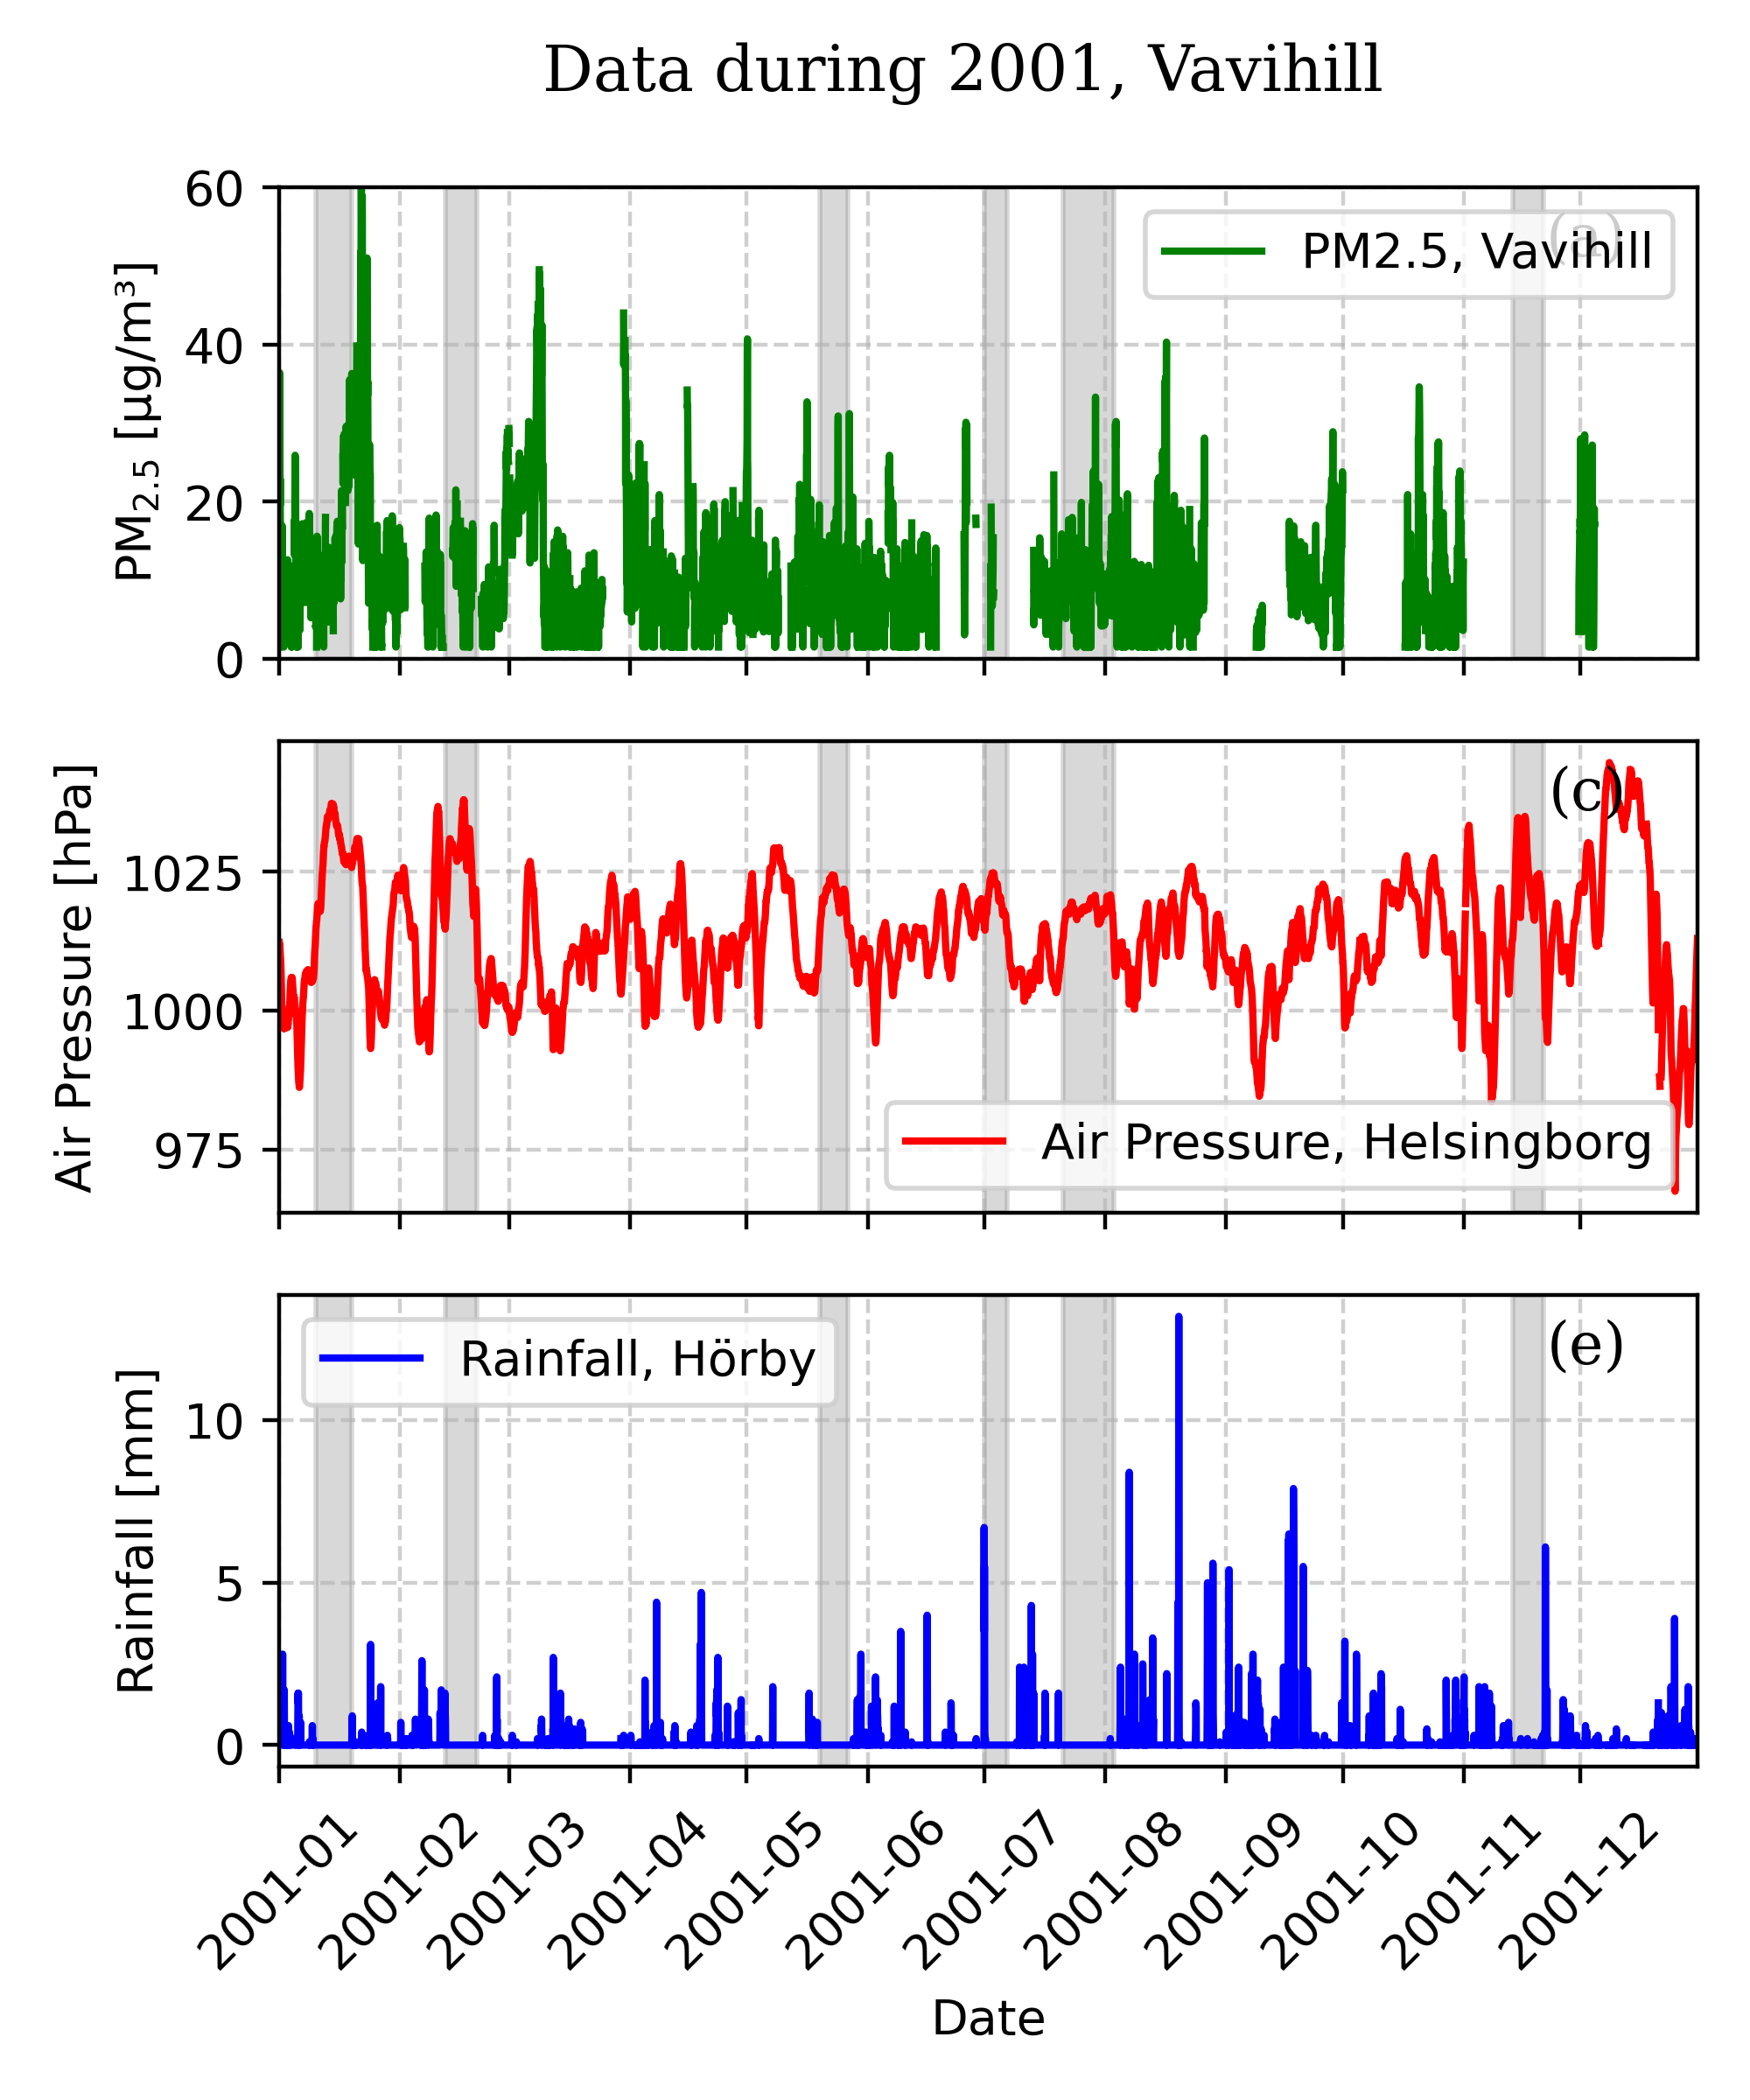
\includegraphics[width=\textwidth]{Figures/Vavihill_plot_20010101_20011231.png}
        \label{fig:2001Vavihill}
    \end{subfigure}
    \hfill
    \begin{subfigure}[b]{0.49\textwidth}
        \centering
        \includegraphics[width=\textwidth]{Figures/Malmö_plot_20010101_20011231.png}
        \label{fig:2001Malmö}
    \end{subfigure}
    \caption{Example plots displaying the air pressure, \PM concentrations, and rainfall during the year 2001. The periods which were indicated as periods of high-pressure blocking events are shown in gray. This displays a normal yearly distribution of high-pressure blocking events using the described method.}
    \label{fig:2001}
\end{figure}

The average change in \PM concentrations during periods of high-pressure blocking can be seen in \autoref{fig:Meanplot_Comparison}. The data is compared with the \PM mean taken from periods without high-pressure blocking events. An increase in \PM concentrations can be seen in Malmö from \SI{10}{\micro\gram\per\meter\cubed} to a maximum of \SI{21}{\micro\gram\per\meter\cubed} at day thirteen, and an increase from \SI{7}{\micro\gram\per\meter\cubed} to a maximum of \SI{17}{\micro\gram\per\meter\cubed} at day twelve can be seen in Vavihill. A stronger increase in Malmö is supported by the large $\tau$-value of $\tau=0.80$, and slight lower in Vavihill $\tau=0.71$. The Sen's slope values also indicate a stronger increase in Malmö \SI{2.8e-02}{} compared to \SI{1.9e-02}{} in Vavihill. After the first five days, the number of high-pressure blocking events decreases, which is reflected in the increase in standard deviation. Figure~\ref{fig:Meanplot_Comparison}--\ref{fig:Meanplot_pressure} all provided significant result since all had a p-value approximately equal to 0.


\begin{figure}[H]
    \centering
    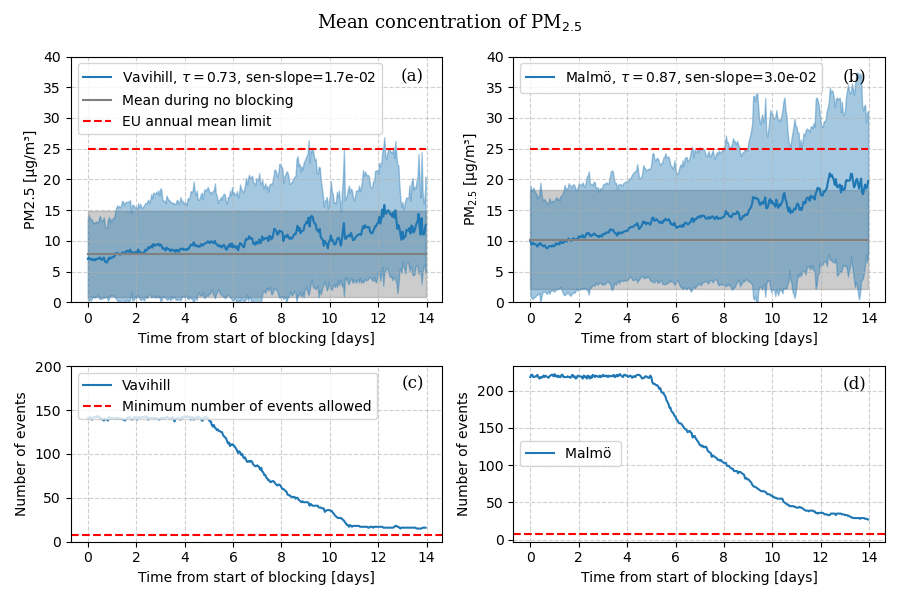
\includegraphics[width=\textwidth]{Figures/Meanplot.png}
    \caption{Comparison of mean \PM  concentrations in Vavihill (a) and Malmö (b), highlighting differences between rural and urban air quality. The shaded region indicates the standard deviation of the data. The number of high-pressure blocking events used in the analysis can be seen in (c) and (d).}
    \label{fig:Meanplot_Comparison}
\end{figure}

\subsubsection{The Change in Aerosol Concentrations Depending on Wind Direction}

The change in \PM concentrations in Vavihill and Malmö for different wind directions can be seen in \autoref{fig:Meanplot_wind}. In the case of Vavihill, 6.7\% of the winds came from the northeast (310° to 70°), 27.7\% from the southeast (70° to 190°), 23.5\% from the west (190° to 310°) and 42.0\% from no specific direction. In the case of Malmö, 8.5\% of the winds came from the northeast (310° to 70°), 24.3\% from the southeast (70° to 190°), 18.5\% from the west (190° to 310°) and 49.2\% from no specific direction. 


One can observe similarities between the aerosol concentrations depending on wind directions for Vavihill and Malmö, although a larger increase can be observed in Malmö. When the wind filter was applied for the northeast direction, no strong increase or high levels of \PM were detected, as supported by the $\tau$-values being under 0.5 for both locations (a-b). In Vavihill for southeastern direction yielded $\tau=0.43$, however there is a clear increase until day nine, where the levels suddenly drop (c). The $\tau$-value for the first nine days is $\tau=0.68$, showing a clear increase. The southeastern direction for Malmö yielded a high $\tau$-value of $\tau=0.64$ and mean concentration exceeding the EU annual mean limit with a maximum concentration of \SI{26}{\micro\gram\per\meter\cubed}(d). For the western wind direction, an increase in \PM can be seen in Vavihill as supported by $\tau=0.62$ (e). The western wind direction for Malmö showed an increase until day eight, where it suddenly drops. Although elevated levels can be seen on day eight, one must note that the spread of the values is large (f). 

\begin{figure}[H]
    \centering
    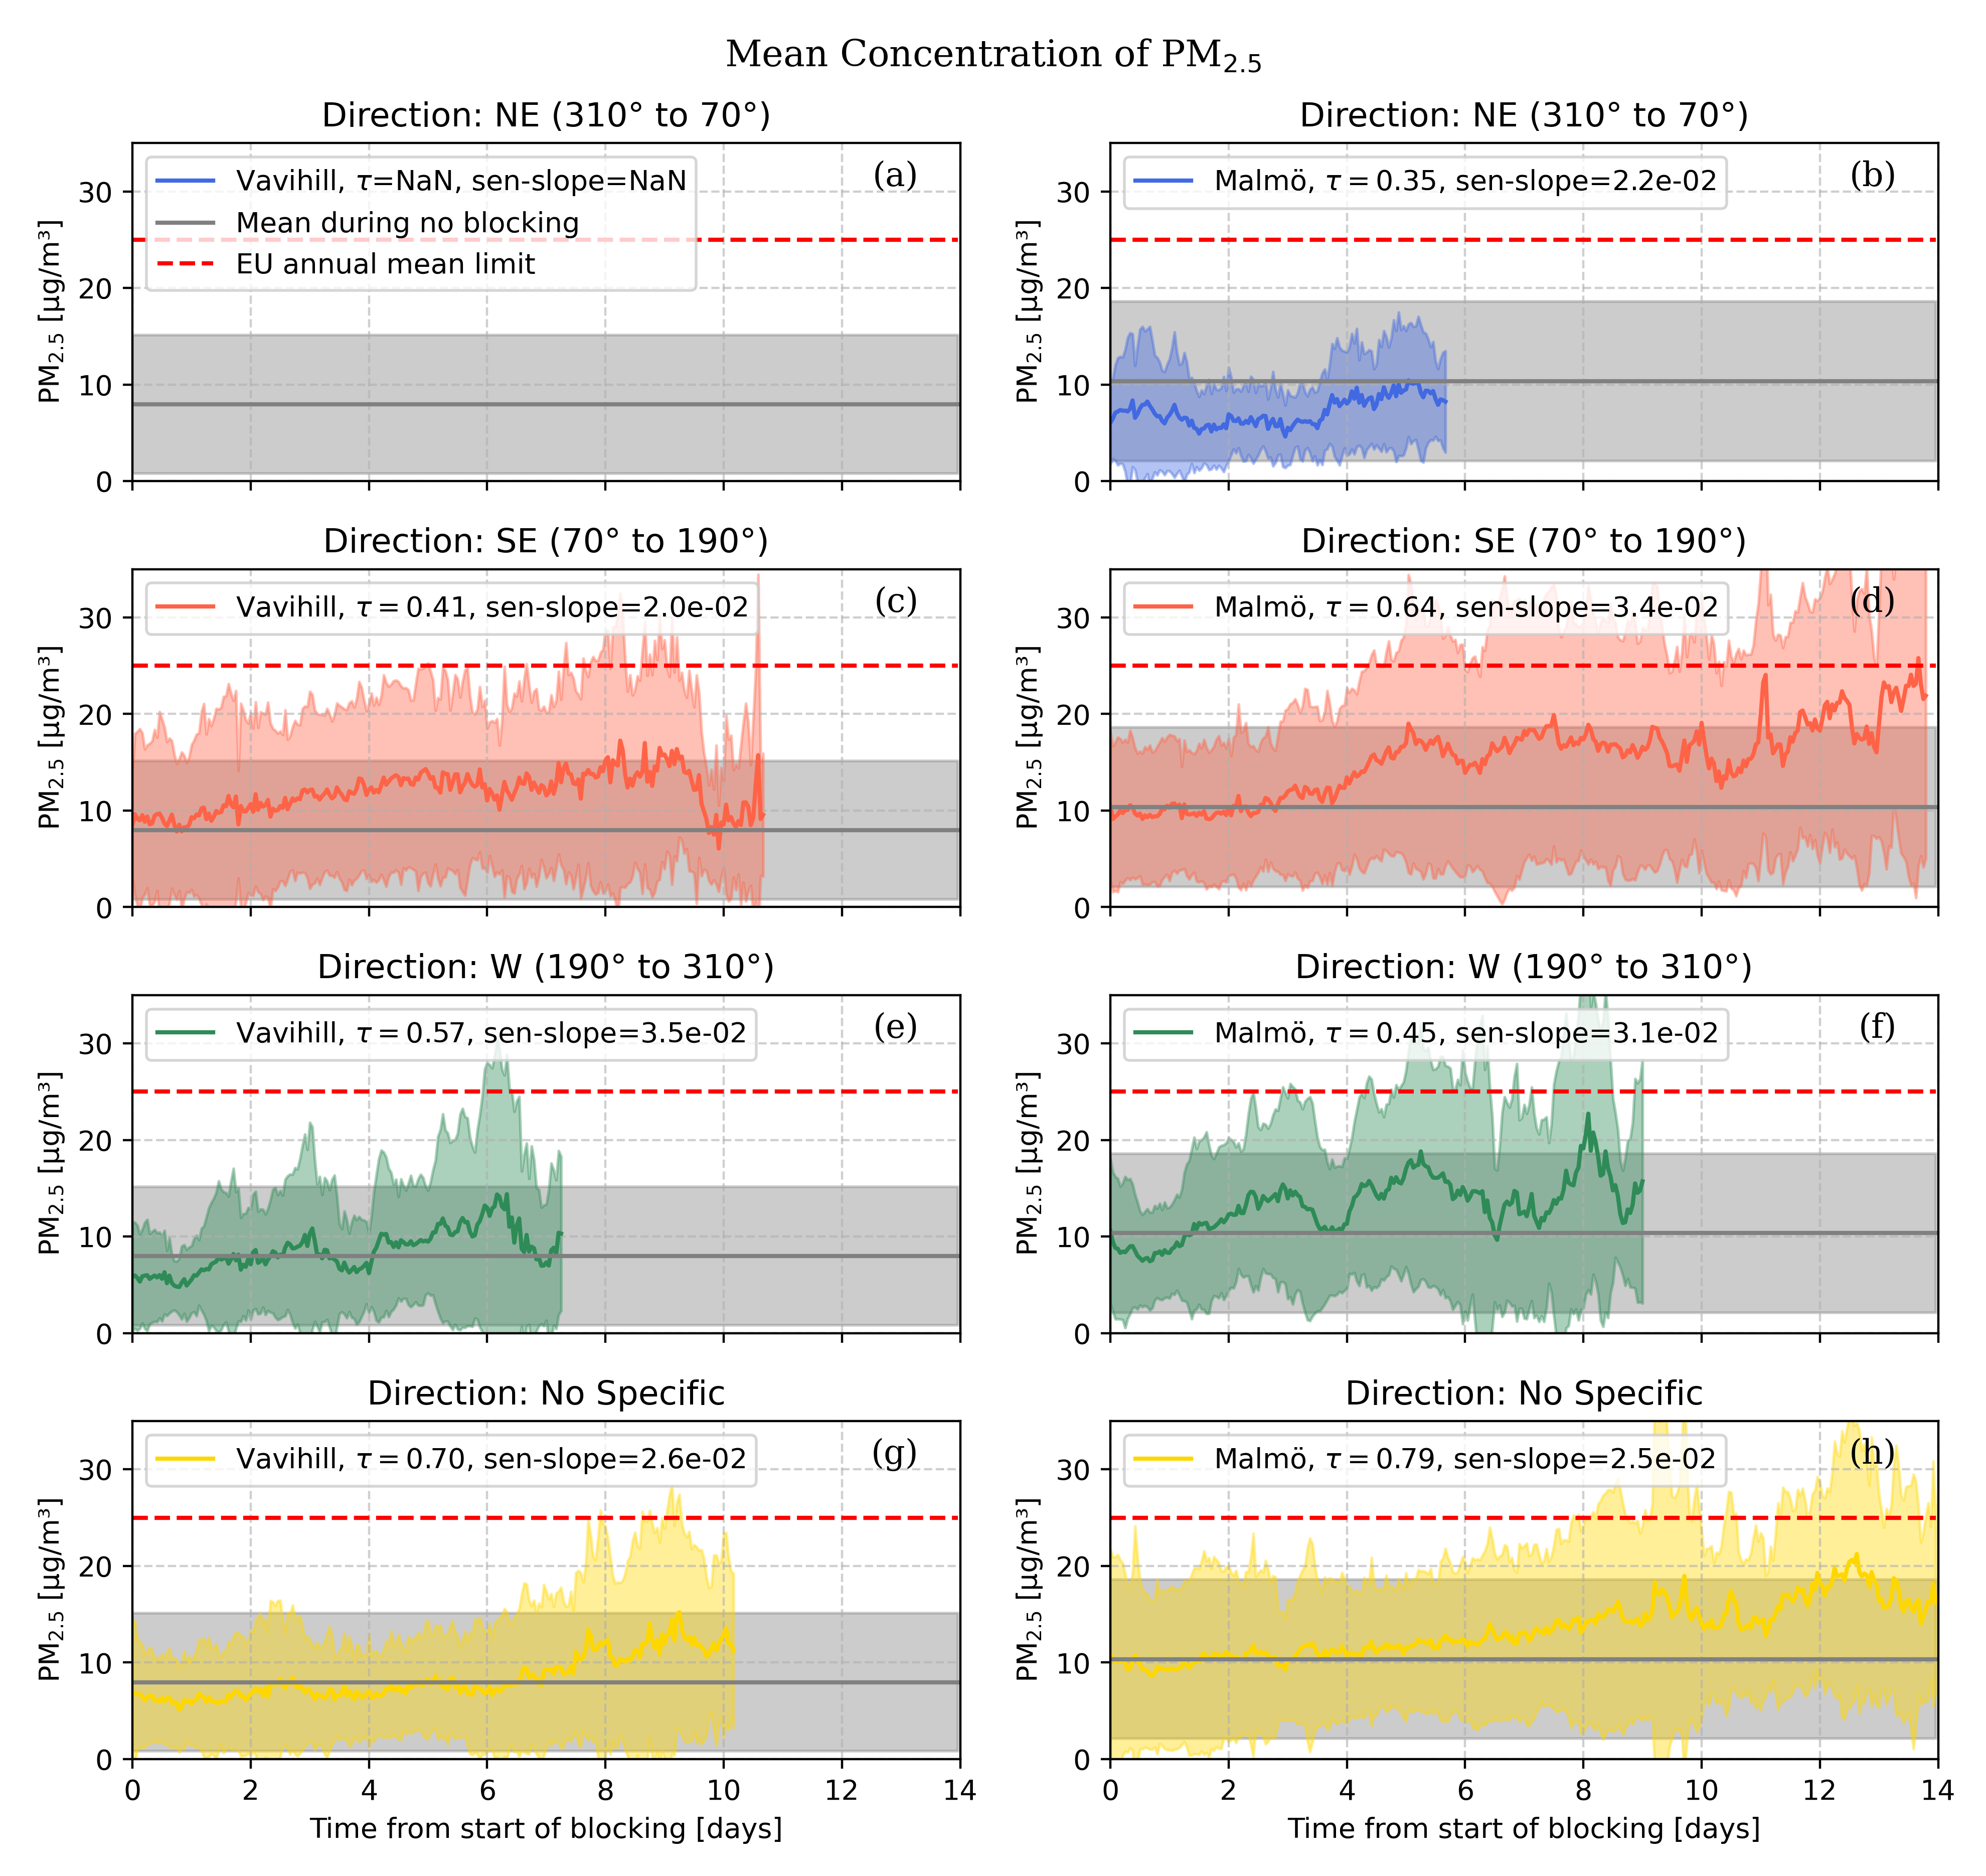
\includegraphics[width=\textwidth]{Figures/Meanplot_dir.png}
    \caption{Plots showing how \PM concentrations in Vavihill and Malmö evolve for different wind directions. A minimum number of blocking events was still put to eight, resulting in some directions having very little data.}
    \label{fig:Meanplot_wind}
\end{figure}

 

\subsubsection{The Change in Aerosol Concentrations Depending on Season}
The seasonal change in concentrations of \PM can be seen in \autoref{fig:Meanplot_seasonal}. In the case of Vavihill 19.0\% of the blocking events occurred during the winter, 31.0\% during the spring, 21.4\% during the summer and 28.6\% during the autumn. In the case of Malmö, 19.6\% of the blocking events occurred during the winter, 33.3\% during the spring, 17.4\% during the summer and 29.7\% during the autumn. 

From \autoref{fig:Meanplot_seasonal} e-f, it is clear that the concentration during the summer for both Vavihill and Malmö does not indicate an increase nor high levels of \PM. A slight increase can be seen in the case of spring for both locations in (c) and (d), with Vavihill going from \SI{9}{\micro\gram\per\meter\cubed} to a maximum of \SI{14}{\micro\gram\per\meter\cubed} and Malmö from \SI{10}{\micro\gram\per\meter\cubed} to a maximum of \SI{14}{\micro\gram\per\meter\cubed}. A larger increase can be seen during the autumn (g-h), where high levels of \PM can be observed towards the end of the period, with Vavihill going from \SI{10}{\micro\gram\per\meter\cubed} to a maximum of \SI{20}{\micro\gram\per\meter\cubed} and Malmö from \SI{11}{\micro\gram\per\meter\cubed} to a maximum of \SI{24}{\micro\gram\per\meter\cubed}. The winter in Vavihill and Malmö indicates an increase in the \PM concentrations, although the standard deviation indicates highly dispersed data (a-b). Although the $\tau$-value during the winter in Malmö is relatively low, Sen's slope indicate a stronger increase. From the graph one can see an increase in \PM concentrations, although the levels seem to decrease towards the end of the period. 

\begin{figure}[H]
    \centering
    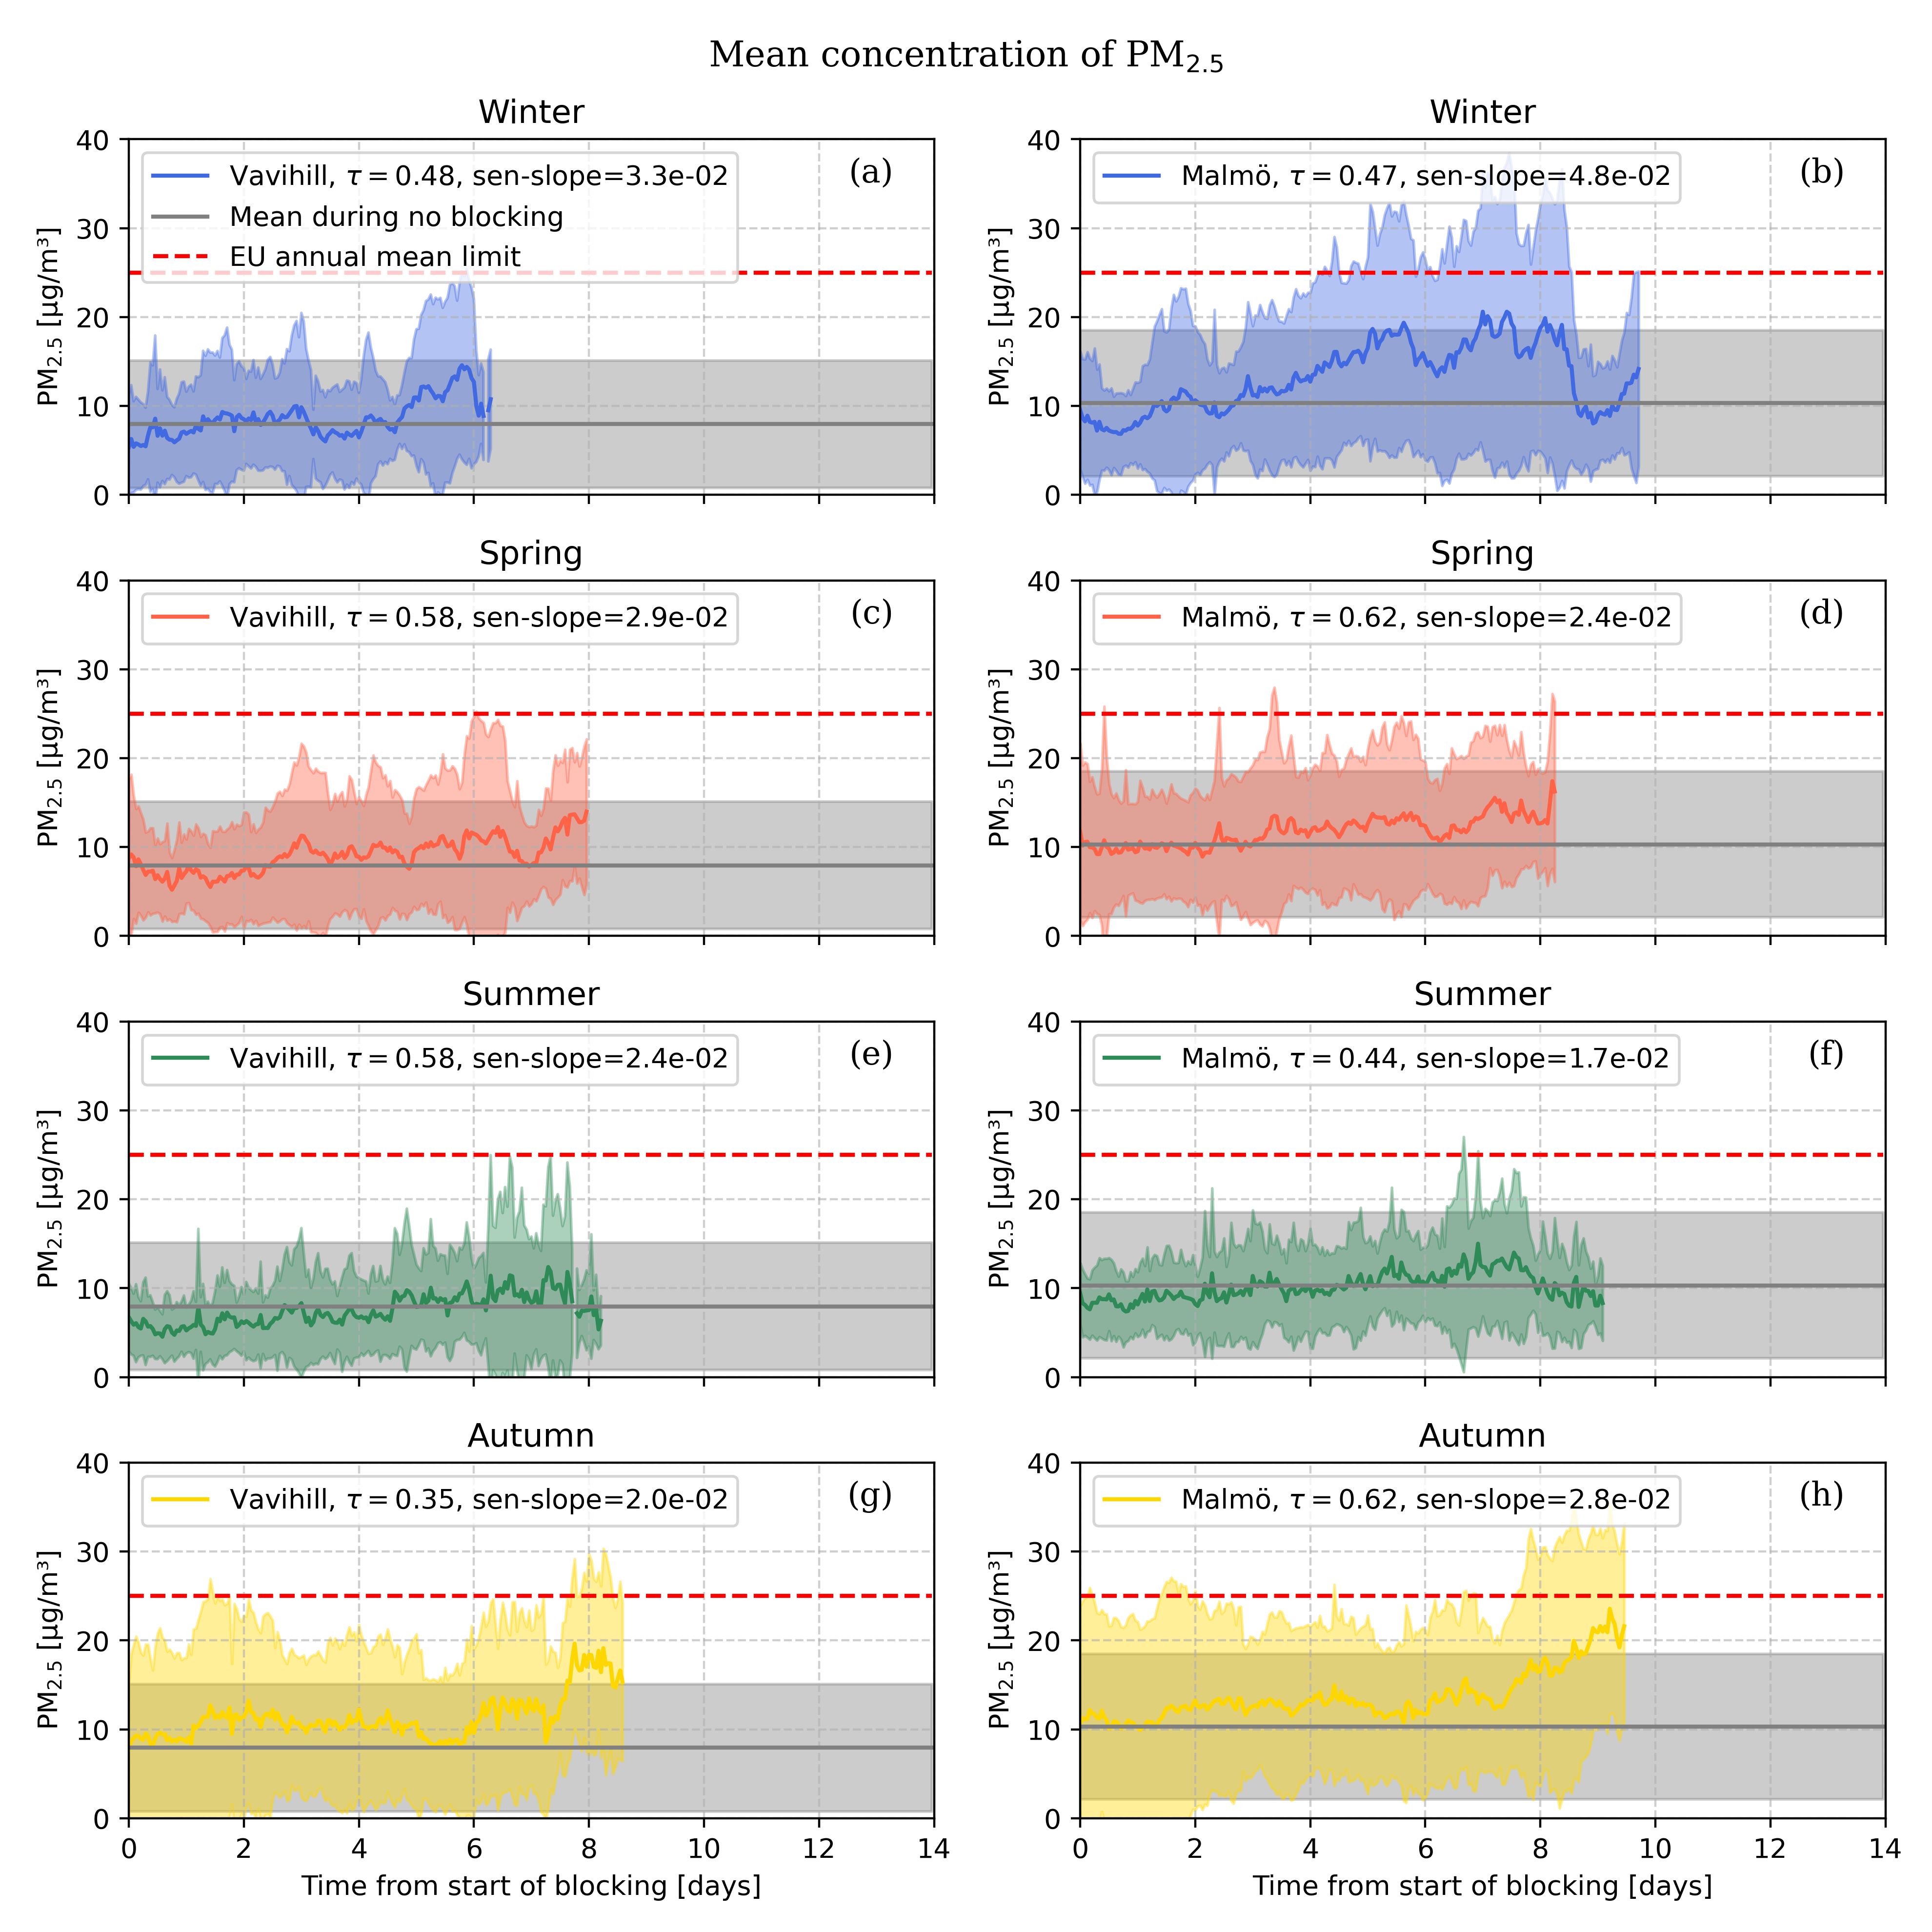
\includegraphics[width=\textwidth]{Figures/Meanplot_seasonal.png}
    \caption{Plots showing \PM concentrations in Vavihill and Malmö for different seasons. }
    \label{fig:Meanplot_seasonal}
\end{figure}
 

\subsubsection{The Change in Aerosol Concentrations Depending on Pressure Strength}
The increase in \PM  concentrations depending on the strength of the high-pressure blocking event can be seen in \autoref{fig:Meanplot_pressure}. In the case of Vavihill, 21.0\% of the blocking events occurred with a mean pressure below 1020 hPa 47.9\% occurred between 1020 and 1025 hPa and 31.1\% occurred with a mean pressure over 1025hPa. In the case of Malmö, 16.4\% of the blocking events occurred with a mean pressure below 1020 hPa 49.2\% occurred between 1020 and 1025 hPa and 34.4\% occurred with a mean pressure over 1025hPa.


From the plots, we can observe similar behaviour in the two locations. In the case of weaker high-pressure blocking events no clear monotonic increase nor highly elevated levels of \PM can be seen, as seen in (a) and (b). In the case of medium strong high-pressure blocking events we see a stronger increase in the case of Vavihill $\tau=0.59$ and weaker in Malmö from $\tau=0.33$. However when observing both plots one can see an increase for both plots around day nine, as seen in (c) and (e). In the case of stronger high-pressure blocking events we see a strong increase in the case of Malmö and in Vavihill, although the increase in Vavihill is slightly less clear. When viewing the plots one can observe that the levels of \PM in the case of Vavihill and Malmö exceed the normal range at day 13, where the mean reach the EU annual mean limit for Malmö. In Vavihill the values went from \SI{8}{\micro\gram\per\meter\cubed} to a maximum of \SI{17}{\micro\gram\per\meter\cubed} and in Malmö they went from \SI{12}{\micro\gram\per\meter\cubed} to a maximum of \SI{27}{\micro\gram\per\meter\cubed}. 


\begin{figure}[H]
        \centering
        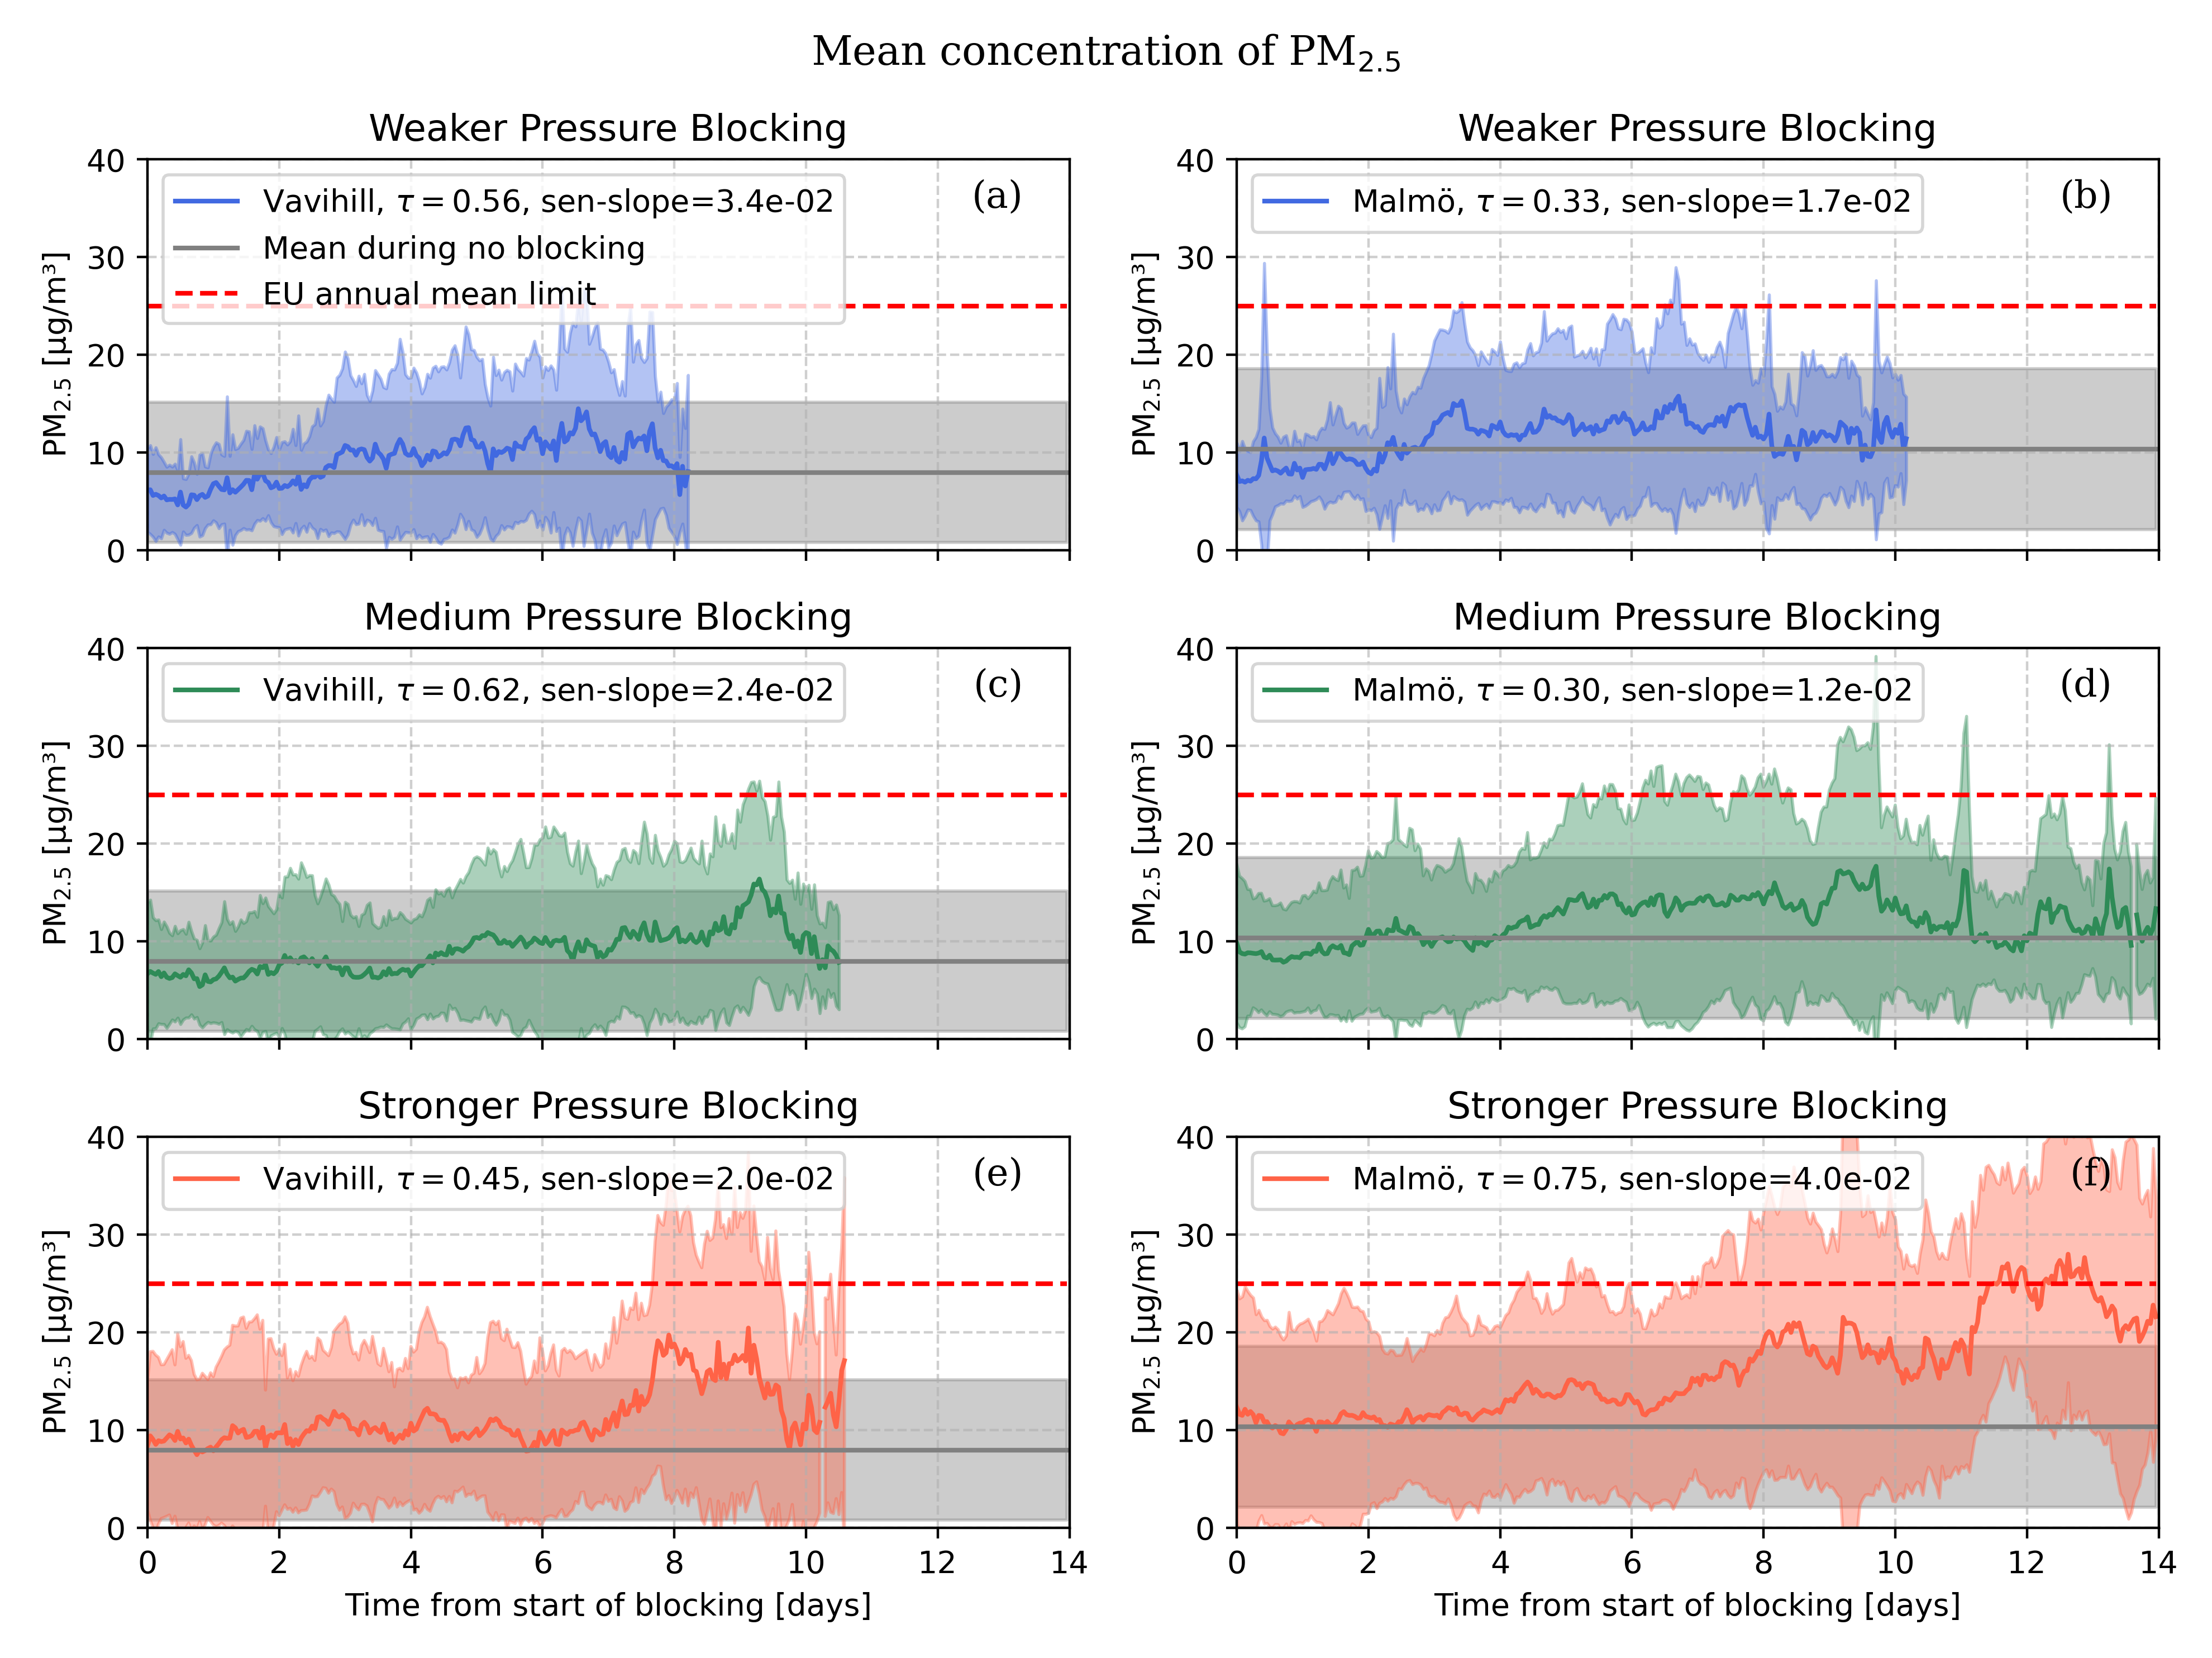
\includegraphics[width=\textwidth]{Figures/Meanplot_pressure.png}
        \caption{Plots showing \PM concentrations in Vavihill and Malmö for different pressure strengths for high-pressure blocking events.}
        \label{fig:Meanplot_pressure}
\end{figure}

 

From Figure~\ref{fig:Meanplot_Comparison}--\ref{fig:Meanplot_pressure} it is clear that the high elevations of \PM occur after eight to thirteen days. These results indicates that prolonged periods of high-pressure blocking events indicate an accumulative increase of \PM, which can be seen in \autoref{fig:Meanplot_Comparison} where we see that the combination of all the other plots resulted in a steady increase in the case of Malmö, and an increase in the case of Vavihill. The only case were we do not see an increase is when the wind direction is from the northeast (see \autoref{fig:Meanplot_wind} a-b), which is not very common. This result indicates that for high-pressure blocking events we observe an increase in the concentration of \PM after eight to thirteen days regardless of the type of high-pressure blocking event, even though different types of high-pressure blocking events may differ in their specific increase.

\subsection{The Frequency of High-Pressure Blocking Events}
The last task was to determine whether high-pressure blocking events have become more common. When observing the number of high-pressure blocking events per year, no significant change in frequency could be seen (see \autoref{fig:number_of_blockings}). Since the highest levels of \PM  occurred toward the end of the events (see Figure~\ref{fig:Meanplot_Comparison}--\ref{fig:Meanplot_pressure}), the frequency of longer high-pressure blocking events was also examined. However, no increase could be observed in any of the cases. More interestingly a small decrease can be observed from the $\tau$-values and the Sen's slope values. However one must note that the p-values are much larger here than Figure~\ref{fig:Meanplot_Comparison}--\ref{fig:Meanplot_pressure}, indicating a more random system. 

\begin{figure}[H]
    \centering
    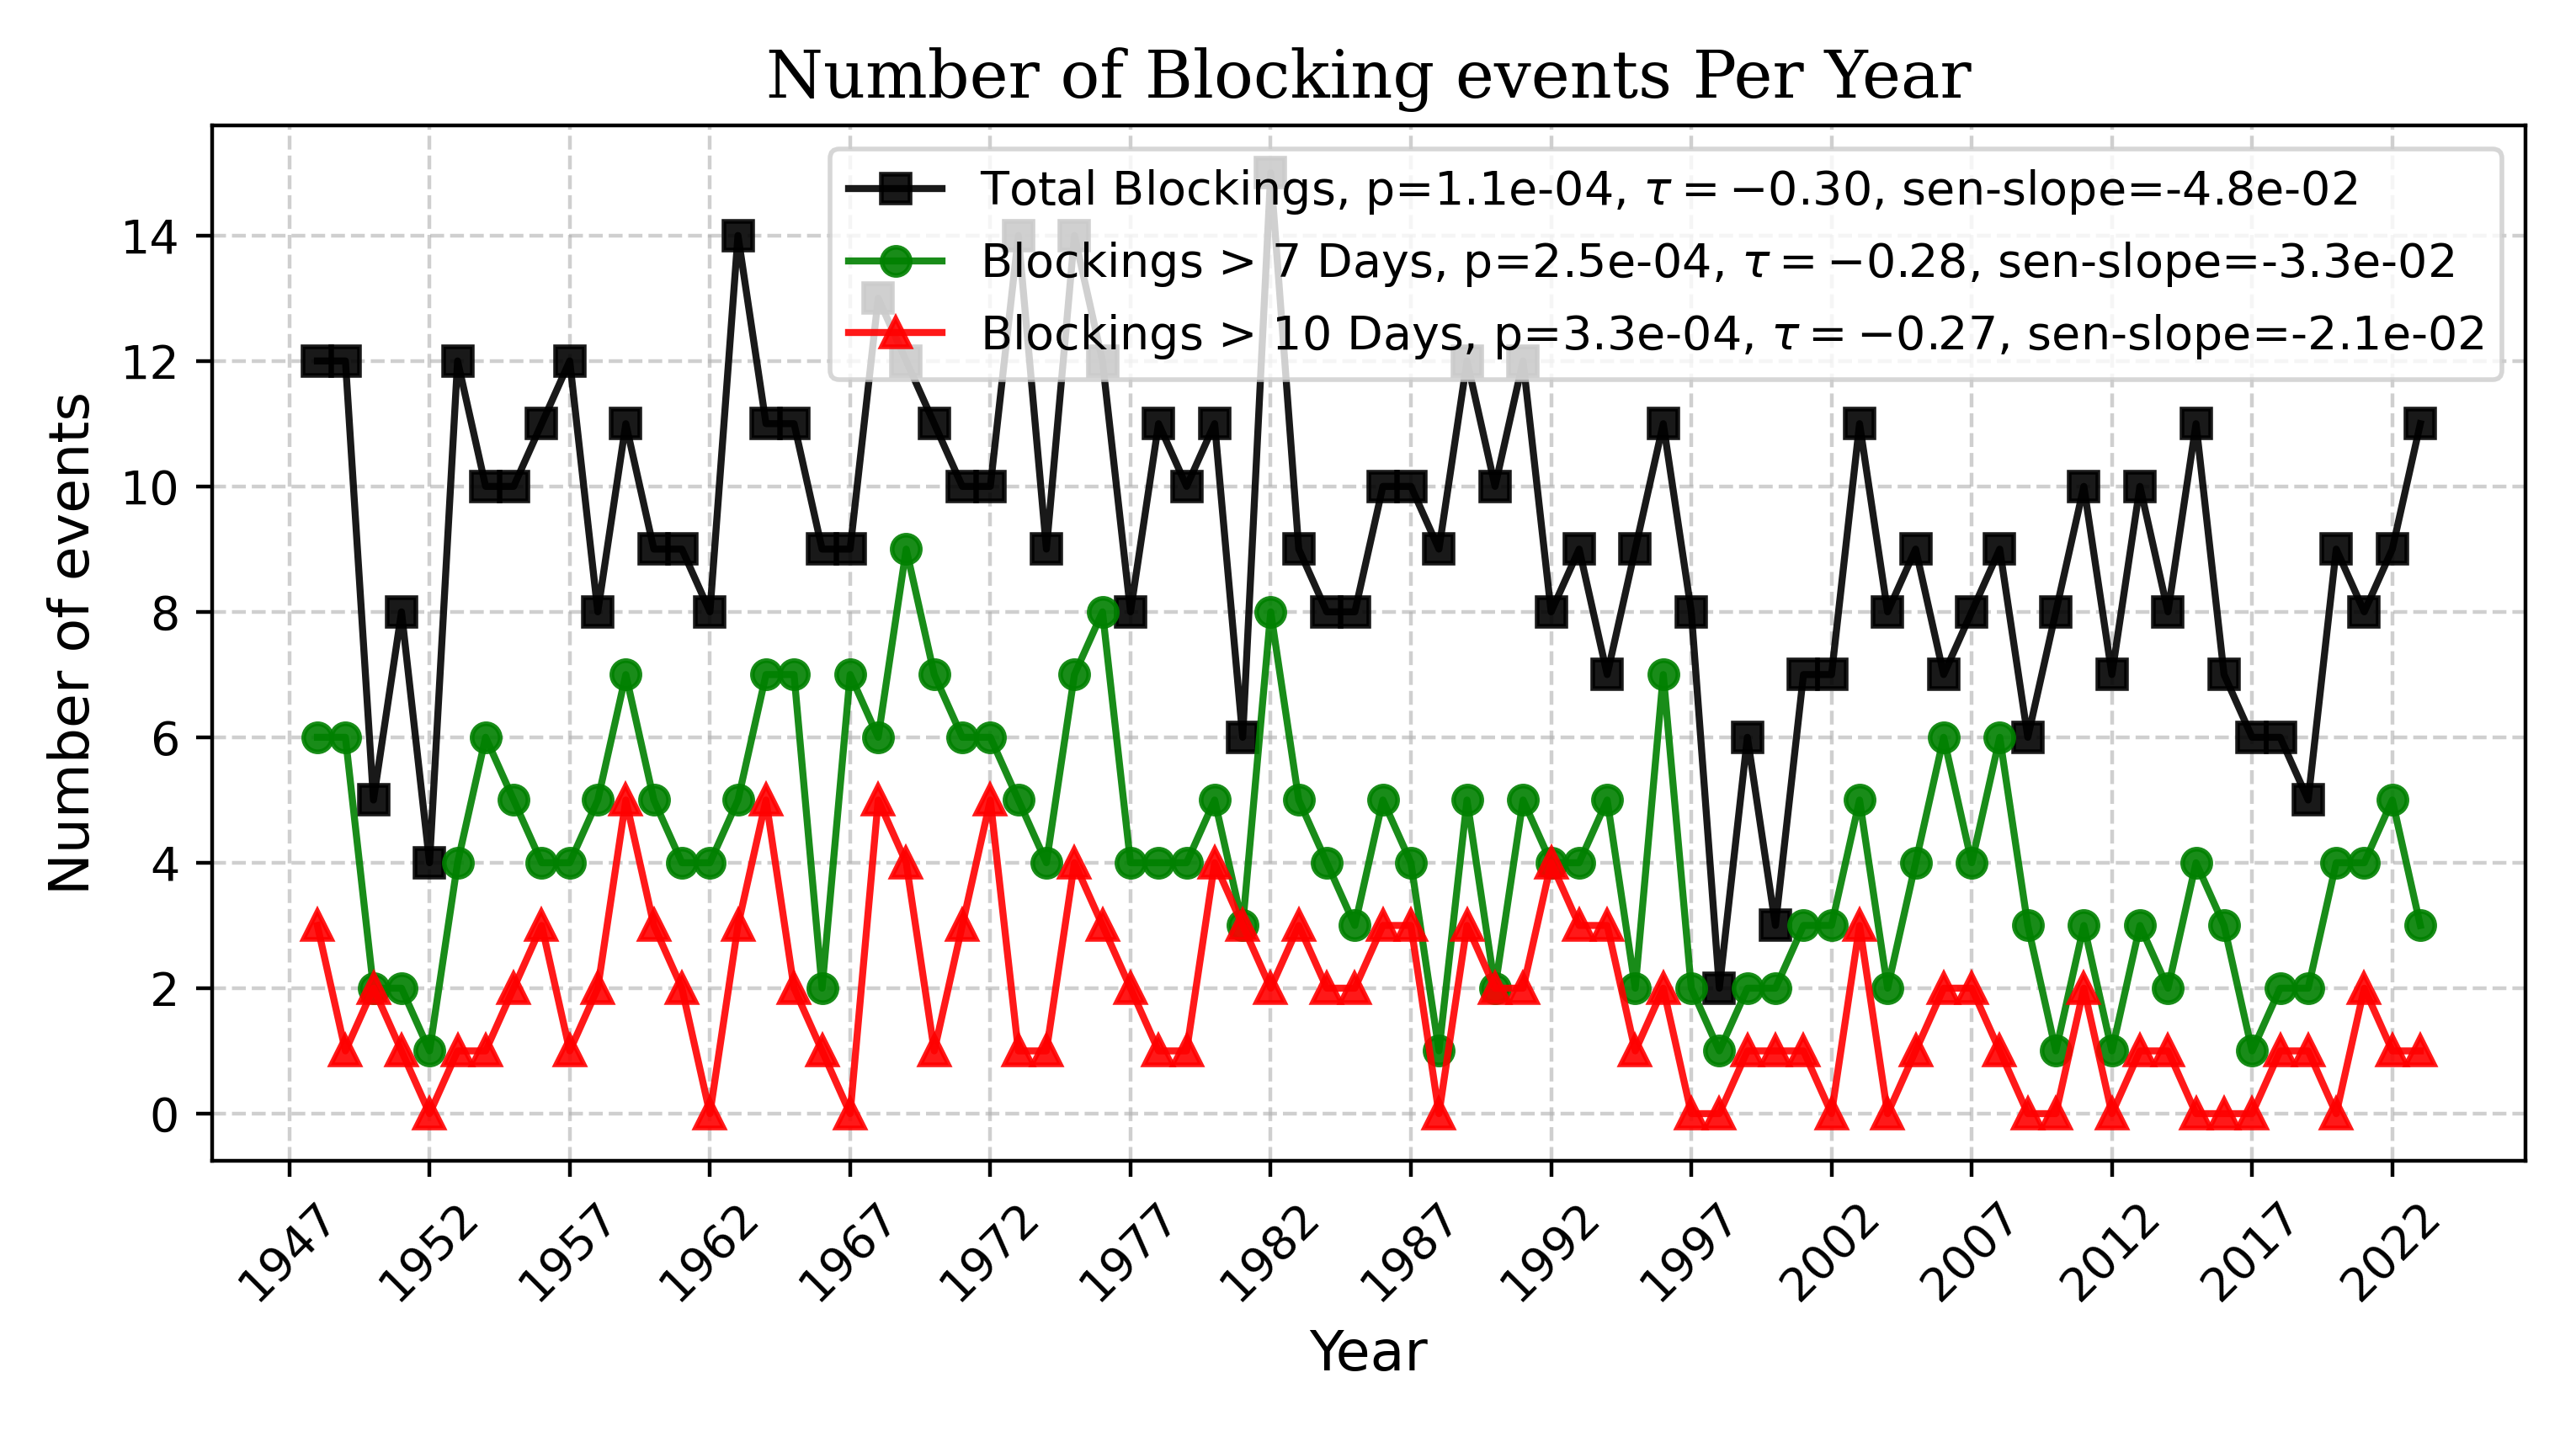
\includegraphics[width=0.7\textwidth]{Figures/BlockingsPerYear.png}
    \caption{fig: This plots shows the change in frequency of high-pressure blocking events. The plots also indicates the change in events longer than seven and ten days. }
    \label{fig:number_of_blockings}
\end{figure}

In \autoref{fig:Number_of_Blocking_Days_Per_Year}, the number of days with high-pressure blocking events per year can be seen. Here, the total, seasonal, and pressure strength dependence can be observed. The reason for not including the directional dependence is that no wind data was available for this period. Even here a slight decrease can be seen in most plots, especially the total blocking days per year (h). 


\begin{figure}[H]
    \centering
    \includegraphics[width=\textwidth]{Figures/blocking_days_per_year_all.png}
    \caption{Plots showing the change in frequency of days under high-pressure blocking events. The number of days under a high-pressure blocking event each year, during each season, and for different pressure strengths can also be seen.}
    \label{fig:Number_of_Blocking_Days_Per_Year}
\end{figure}

When observing slight decline of the frequency of the high-pressure blocking events in \autoref{fig:number_of_blockings} and \autoref{fig:Number_of_Blocking_Days_Per_Year} one must note that the low $\tau$-values indicate that the trend is not monotonic. Furthermore, the large p-values indicate that the trend is not as non-random as seen in the mean aerosol concentration plots observed in Figures~\ref{fig:Meanplot_Comparison}--\ref{fig:Meanplot_pressure}. This indicates that this trend is more likely caused to randomness, and should not be seen as a result. However, one can observe that no type of high-pressure blocking events has become more common during the last 74 years. This is an interesting result since the opposite has been found in in western Europe \cite{lupoAtmosphericBlockingEvents2020}. 
